%%%%%%%%%%%%%%%%%%%%%%%%%%%%%%%%%%%%%%%%%%%%%%%%%%%%%%%%%%%%%%%%%%%%%%%%%%%%%%%%
\chapter{Introduction}
%%%%%%%%%%%%%%%%%%%%%%%%%%%%%%%%%%%%%%%%%%%%%%%%%%%%%%%%%%%%%%%%%%%%%%%%%%%%%%%%

This is 'Boost.Graph Cookbook 1: Basics', version 3.3.

\subsection{Why this tutorial}

I needed this tutorial already in 2006, when I started experimenting with
Boost.Graph.
More specifically, I needed a tutorial that:

\begin{itemize}
  \item Orders concepts chronologically
  \item Increases complexity gradually
  \item Shows complete pieces of code
\end{itemize}

What I had were the book \cite{siek2001boost}
and the Boost.Graph website, both did not satisfy these requirements.

\subsection{Tutorial style}

\paragraph{Readable for beginners}

This tutorial is aimed at the beginner programmer.
This tutorial is intended to take the reader to the level of understanding
the book \cite{siek2001boost}
and the Boost.Graph website require.
It is about basic graph manipulation, not the more advanced graph algorithms.
 
\paragraph{High verbosity}

This tutorial is intended to be as verbose, such that a beginner should
be able to follow every step, from reading the tutorial from beginning
to end chronologically.
Especially in the earlier chapters, the rationale behind the code presented
is given, including references to the literature.
Chapters marked with $\triangle$ are optional, 
less verbose and bring no new information to the storyline.

\paragraph{Repetitiveness}

This tutorial is intended to be as repetitive, such that a beginner can
 spot the patterns in the code snippets their increasing complexity.
 Extending code from this tutorial should be as easy as extending the patterns.

\paragraph{Index}

In the index, I did first put all my long-named functions there literally,
but this resulted in a very sloppy layout.
Instead, the function 'do\_something' can be found as 'Do something' in
the index.
On the other hand, STL and Boost functions like 'std::do\_something' and
'boost::do\_something' can be found as such in the index.

\subsection{Coding style}

\paragraph{Concept}

For every concept, I will show

\begin{itemize}
    \item a function that achieves a goal, 
      for example \verb;create_empty_undirected_graph;
    \item{
      a test case of that function, 
      that demonstrates how to use the function, for example
      \verb;create_empty_undirected_graph_test;
    }
    \item Three
\end{itemize}

\paragraph{C++14}

All coding snippets are taken from compiled and tested C++14 code.
I chose to use C++14 because it was available to me on all local and remote
computers.
Next to this, it makes code even shorter then just C++11.

\paragraph{Coding standard}

I use the coding style from the Core C++ Guidelines.
At the time of this writing, the Core C++ Guidelines were still in early
development, so I can only hope the conventions I then chose to follow
are still Good Ideas.

\paragraph{No comments in code}

It is important to add comments to code.
In this tutorial, however, I have chosen not to put comments in code, as
I already describe the function in the tutorial its text.
This way, it prevents me from saying the same things twice.

\paragraph{Trade-off between generic code and readability}

It is good to write generic code.
In this tutorial, however, I have chosen my functions to have no templated
arguments for conciseness and readability.
For example, a vertex name is std::string, the type for if a vertex is
selected is a boolean, and the custom vertex type is of type \verb;my_custom_vertex;.
I think these choices are reasonable and that the resulting increase in
readability is worth it.

\paragraph{Long function names}

I enjoy to show concepts by putting those in (long-named) functions.
These functions sometimes border the trivial, by, for example, only calling
a single Boost.Graph function.
On the other hand, these functions have more English-sounding names, resulting
in demonstration code that is readable.
Additionally, they explicitly mention their return type (in a simpler way),
which may be considered informative.

\paragraph{Long function names and readability}

Due to my long function names and the limitation of 50 characters per line,
sometimes the code does get to look a bit awkward.
I am sorry for this.

\paragraph{Use of auto}

I prefer to use the keyword auto over doubling the lines of code for using
statements.
Often the \verb;do; functions return an explicit data type, these can be used
for reference.
Sometime I deduce the return type using decltype and a function with the
same return type.
When C++17 gets accessible, I will use \verb;decltype(auto);
If you really want to know a type, you can use the \verb;get_type_name; function
(chapter \ref{subsec:get_type_name})

\subparagraph{Explicit use of namespaces}

On the other hand, I am explicit in the namespaces of functions and classes
I use, so to distinguish between types like \verb;std::array; and \verb;boost::array;.
Some functions (for example, \verb;get;) reside 
in the namespace of the graph to work on.
In this tutorial, this is in the global namespace.
Thus, I will write \verb;get;, instead of \verb;boost::get;, 
as the latter does not compile.

\paragraph{Use of STL algorithms}

I try to use STL algorithms wherever I can.
Also you should prefer algorithm calls over hand-written 
for-loops (\cite{stroustrup1997}, chapter 18.12.1 and \cite{meyers2005effective}, item 43).
Sometimes using these algorithms becomes a burden on the lines of code.
This is because in C++11, a lambda function argument (use by the algorithm)
must have its data type specified.
It may take multiple lines of \verb;using; statements being able to do so.
In C++14 one can use \verb;auto; there as well.
So, only if it shortens the number of lines significantly, I use raw for-loops,
even though you shouldn't.

\paragraph{Re-use of functions}

The functions I develop in this tutorial are re-used from that moment on.
This improves to readability of the code and decreases the number of lines.

\paragraph{Tested to compile}

All functions in this tutorial are tested to compile using GitHub Actions in
both debug and release mode.

\paragraph{Tested to work}

All functions in this tutorial are tested, using the Boost.Test library.
GitHub Actions calls these tests after each push to the repository.

\paragraph{Availability}

The code, as well as this tutorial, can be downloaded from the GitHub at
\url{www.github.com/richelbilderbeek/boost_graph_cookbook_1}.

\subsection{License}

This tutorial is licensed under Creative Commons license 4.0.
All C++ code is licensed under GPL 3.0.

\begin{figure}[!htbp]
  \includegraphics[]{CC-BY-SA_icon.png}
  \caption{
    Creative Commons license 4.0
  }
  \label{fig:license}
\end{figure}

\subsection{Feedback}

This tutorial is not intended to be perfect yet.
For that, I need help and feedback from the community.
All referenced feedback is welcome, as well as any constructive feedback.

I have tried hard to strictly follow the style as described above.
If you find I deviated from these decisions somewhere, I would be grateful
if you'd let know.
Next to this, there are some sections that need to be coded or have its
code improved.

\subsection{Acknowledgements}


These are users that improved this tutorial and/or the code behind this
tutorial, in chronological order:

\begin{itemize}
  \item m-dudley, \url{http://stackoverflow.com/users/111327/m-dudley}
  \item E. Kawashima
  \item mat69, \url{https://www.reddit.com/user/mat69}
  \item danielhj, \url{https://www.reddit.com/user/danieljh}
  \item sehe, \url{http://stackoverflow.com/users/85371/sehe}
  \item cv\_and\_me, \url{http://stackoverflow.com/users/2417774/cv-and-he}
  \item mywtfmp3
\end{itemize}

\subsection{Outline}

The chapters of this tutorial are also like a well-connected graph.
To allow for quicker learners to skim chapters, or for beginners looking
to find the patterns.

The distinction between the chapter is in the type of edges and vertices.
They can have:

\begin{itemize}
  \item no properties: 
    see chapter \ref{sec:Building-graphs-without-properties}
  \item have a bundled property: 
    see chapter \ref{sec:Building-graphs-with-bundled-vertices}
\end{itemize}

Pivotal chapters are chapters like 'Finding the first vertex with ...', as
this opens up the door to finding a vertex and manipulating it.

All chapters have a rather similar structure in themselves, as depicted
in figure \ref{fig:The-relations-between-subchapters}.

\begin{figure}[!htbp]
  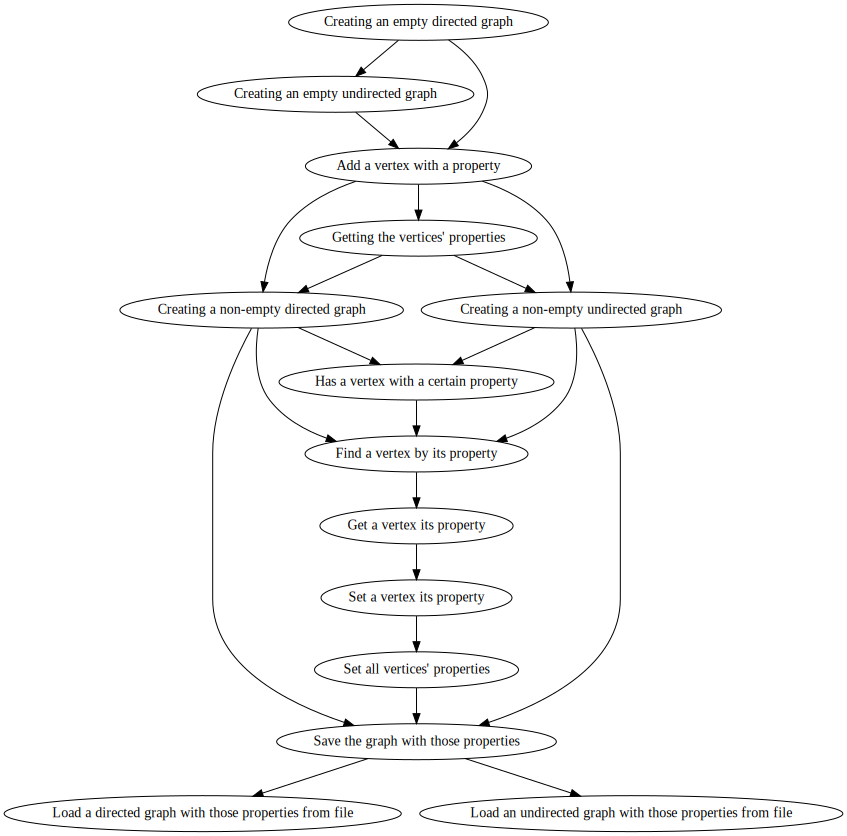
\includegraphics[width=\textwidth]{create_tutorial_subchapters_graph.png}
  \caption{
    The relations between sub-chapters
  }
  \label{fig:The-relations-between-subchapters}
\end{figure}

There are also some bonus chapters, that I have labeled with a $\triangle$.
These chapters are added I needed these functions myself and adding them
would not hurt.
Just feel free to skip them, as there will be less theory explained.

